\chapter{Diseño e implementación} % Main chapter title

\label{Chapter3} % Change X to a consecutive number; for referencing this chapter elsewhere, use \ref{ChapterX}

\definecolor{mygreen}{rgb}{0,0.6,0}
\definecolor{mygray}{rgb}{0.5,0.5,0.5}
\definecolor{mymauve}{rgb}{0.58,0,0.82}

%%%%%%%%%%%%%%%%%%%%%%%%%%%%%%%%%%%%%%%%%%%%%%%%%%%%%%%%%%%%%%%%%%%%%%%%%%%%%
% parámetros para configurar el formato del código en los entornos lstlisting
%%%%%%%%%%%%%%%%%%%%%%%%%%%%%%%%%%%%%%%%%%%%%%%%%%%%%%%%%%%%%%%%%%%%%%%%%%%%%
\lstset{ %
  backgroundcolor=\color{white},   % choose the background color; you must add \usepackage{color} or \usepackage{xcolor}
  basicstyle=\footnotesize,        % the size of the fonts that are used for the code
  breakatwhitespace=false,         % sets if automatic breaks should only happen at whitespace
  breaklines=true,                 % sets automatic line breaking
  captionpos=b,                    % sets the caption-position to bottom
  commentstyle=\color{mygreen},    % comment style
  deletekeywords={...},            % if you want to delete keywords from the given language
  %escapeinside={\%*}{*)},          % if you want to add LaTeX within your code
  %extendedchars=true,              % lets you use non-ASCII characters; for 8-bits encodings only, does not work with UTF-8
  %frame=single,	                % adds a frame around the code
  keepspaces=true,                 % keeps spaces in text, useful for keeping indentation of code (possibly needs columns=flexible)
  keywordstyle=\color{blue},       % keyword style
  language=[ANSI]C,                % the language of the code
  %otherkeywords={*,...},           % if you want to add more keywords to the set
  numbers=left,                    % where to put the line-numbers; possible values are (none, left, right)
  numbersep=5pt,                   % how far the line-numbers are from the code
  numberstyle=\tiny\color{mygray}, % the style that is used for the line-numbers
  rulecolor=\color{black},         % if not set, the frame-color may be changed on line-breaks within not-black text (e.g. comments (green here))
  showspaces=false,                % show spaces everywhere adding particular underscores; it overrides 'showstringspaces'
  showstringspaces=false,          % underline spaces within strings only
  showtabs=false,                  % show tabs within strings adding particular underscores
  stepnumber=1,                    % the step between two line-numbers. If it's 1, each line will be numbered
  stringstyle=\color{mymauve},     % string literal style
  tabsize=2,	                   % sets default tabsize to 2 spaces
  title=\lstname,                  % show the filename of files included with \lstinputlisting; also try caption instead of title
  morecomment=[s]{/*}{*/}
}

%----------------------------------------------------------------------------------------
\section{Detección facial con TensorFlow y TensorFlow Lite}
\label{section3_1}
Como se explicó en el capitulo \ref{Chapter1}, el objetivo principal de este trabajo es detectar rostros humanos con ayuda de algoritmos de AI. Para esto se deben obtener imagenes digitales con ayuda de una camara, procesarlas y utilizarlas como entrada de una red de modelos de DL capaces de realizar la tarea de deteccion facial. Esta red de modelos de DL fue descrita en el capitulo \ref{Chapter2} y se denomina MTCNN.

Para implementar MTCNN adecuadamente no basta con alimentar P-Net con las imagenes obtenidas por la camara, R-Net con las ventanas candidatas de P-Net y O-Net con las ventanas candidatas de R-Net. Los datos de entrada de cada uno de los modelos de MTCNN deben ser procesados para conseguir el mejor resultado posible, como se muestra en el diagrama de la figura \ref{fig:mtcnn_npipe}.

\begin{figure}[h]
	\centering
	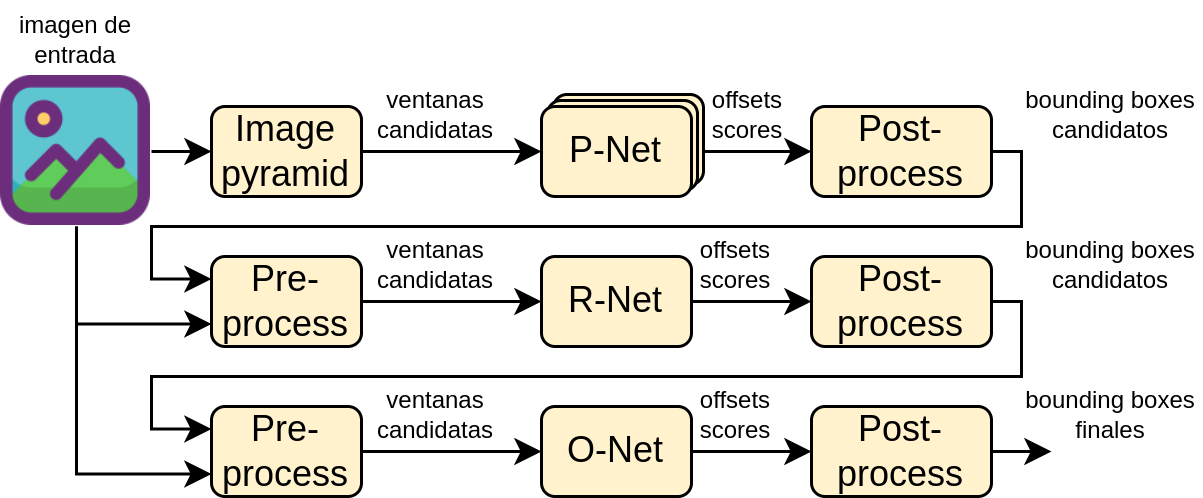
\includegraphics[scale=0.3]{./Figures/mtcnn_npipe.png}
	\caption{\textit{Pipeline} detallado de MTCNN.}
	\label{fig:mtcnn_npipe}
\end{figure}

El diagrama de la figura \ref{fig:mtcnn_npipe} muestra el \textit{pipeline} detallado de la red MTCNN, donde se pueden observar varios bloques de procesamiento, estos son:

\begin{itemize}
	\item \textit{Image pyramid}: genera a partir de la imagen de entrada otras imágenes de escalas inferiores, lo que permite detectar objetos de distintos tamaños. Cada nivel de escala se obtiene mediante la reducción de la escala anterior, por lo que las imágenes en niveles superiores tienen una escala mas baja que las imagenes en niveles inferiores. Después de generadas las imágenes escaladas requeridas de la imagen de entrada estas sirven para alimentar P-Net y así detectar rostros de distintos tamaños.

	\item \textit{Post-process}: en este bloque se procesan los datos de salida generados por P-Net, R-Net y O-Net. El primer subbloque realiza la operación de NMS para reducir la cantidad de ventanas candidatas que tienen solapmiento entre ellas. El segundo subbloque aplica un proceso de calibración que utiliza los \textit{offsets} generados por los modelos para determinar de manera mas precisa las coordenadas de las ventanas candidatas. Finalmente el último subbloque corrige las coordenadas de las ventanas candidatas para que posean dimensiones cuadradas y estén dentro de los límites de la imagen original.
	\begin{figure}[h]
		\centering
		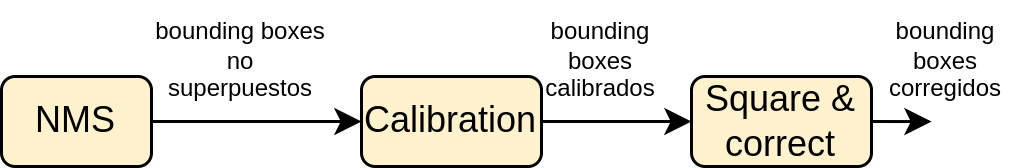
\includegraphics[scale=0.35]{./Figures/mtcnn_postprocess.png}
		\caption{Bloque de postprocesamiento.}
		\label{fig:mtcnn_postprocess}
	\end{figure}
	
	\item \textit{Pre-process}: tiene la función de procesar los datos de entrada para las redes R-Net y O-Net. El primer subbloque genera recortes de la imagen original en función de las coordenadas obtenidas del bloque \textit{post-process}. En el segundo subbloque las imágenes recortadas de entrada son redimensionadas con dimensiones de 24x24 px y 48x48 px, para alimentar R-Net y O-Net respectivamente.`
	\begin{figure}[h]
		\centering
		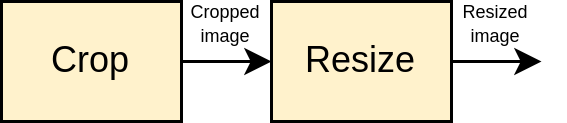
\includegraphics[scale=0.35]{./Figures/mtcnn_preprocess.png}
		\caption{Bloque de preprocesamiento.}
		\label{fig:mtcnn_preprocess}
	\end{figure}

\end{itemize}

P-Net, R-Net y O-Net fueron creados con ayuda de la biblioteca para redes neuronales Keras, que es parte del \textit{core} de TensorFlow, de acuerdo con lo expuesto en \cite{mtcnn_info}. Para P-Net se crearon tantos modelos como escalas utilizadas, en este caso 3, suficientes para detectar rostros a corta distancia. Con las arquitecturas definidas de los modelos el siguiente paso natural en el desarrollo deberia haber sido su entrenamiento con uno o varios \textit{datasets}, pero al ser MTCNN tan popular en el ambito de deteccion facial se pudieron encontrar archivos de tipo HDF (\textit{Hierarchical Data Format}, Formato de Datos Jerárquicos) que contenian los \textit{weights} resultantes de un proceso de entrenamiento anterior. En el siguiente fragmento de codigo se puede observar el código utilizado para crear O-Net.

Para que los modelos obtenidos pudieran ser ejecutados en el hardware objetivo de este trabajo tuvieron que ser convertidos a un formato más liviano y eficiente llamado TensorFlow Lite. El conversor de TensorFlow Lite toma un modelo de TensorFlow y genera un moelo de TensorFlow Lite cuya extensión de archivo es .tflite. La conversión puede seguir 2 caminos según como sean evaluados los modelos de TensorFlow, en la figura \ref{fig:tf2tflite_workflow} se observa el flujo de trabajo del conversor.

\begin{figure}[h]
	\centering
	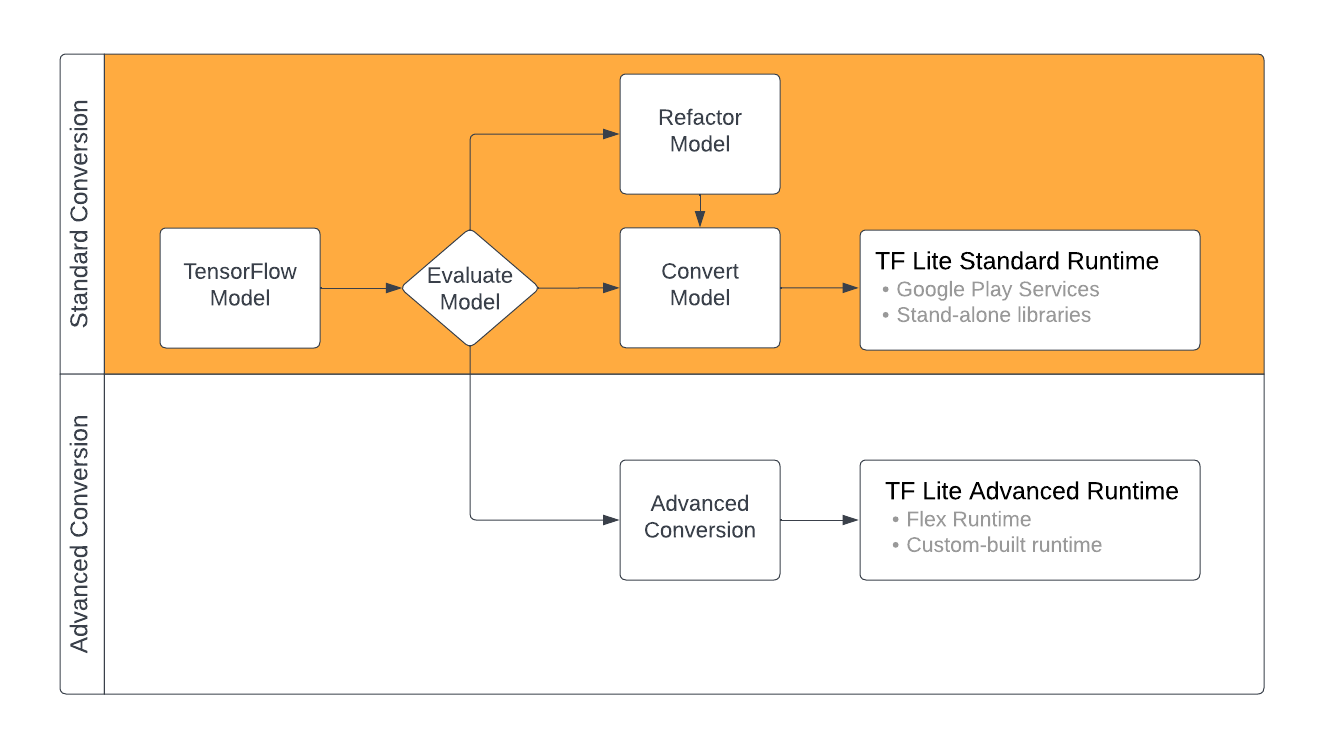
\includegraphics[scale=0.6]{./Figures/tf_convert_workflow_diag.png}
	\caption{Diagrama de flujo de trabajo para la conversion\protect\footnotemark.}
	\label{fig:tf2tflite_workflow}
\end{figure}
\footnotetext{Imagen tomada de: \url{https://www.tensorflow.org/lite/models/convert/}}

Gracias a que todos los operadores utilizados en los modelos de TensorFlow eran compatibles con los operadores de TensorFlow Lite se realizó una conversión estandar, lo que posteriormente facilitó su implementación en el hardware destino.

Durante el proceso de conversión se se aplicaron optimizaciones que responden a una necesidad de reducir aún más el tamaño y la latencia de los modelos. Se realizó una optmización por cuantización, que se refiere a la reducción de la precisión de los numeros usados para representar los parametros de los modelos, los cuales por defecto son flotantes de 32 bits. Las opciones de cuantización para los modelos se tomaron del diagrama de la figura \ref{fig:tf_quantization_tree}.

\begin{figure}[h]
	\centering
	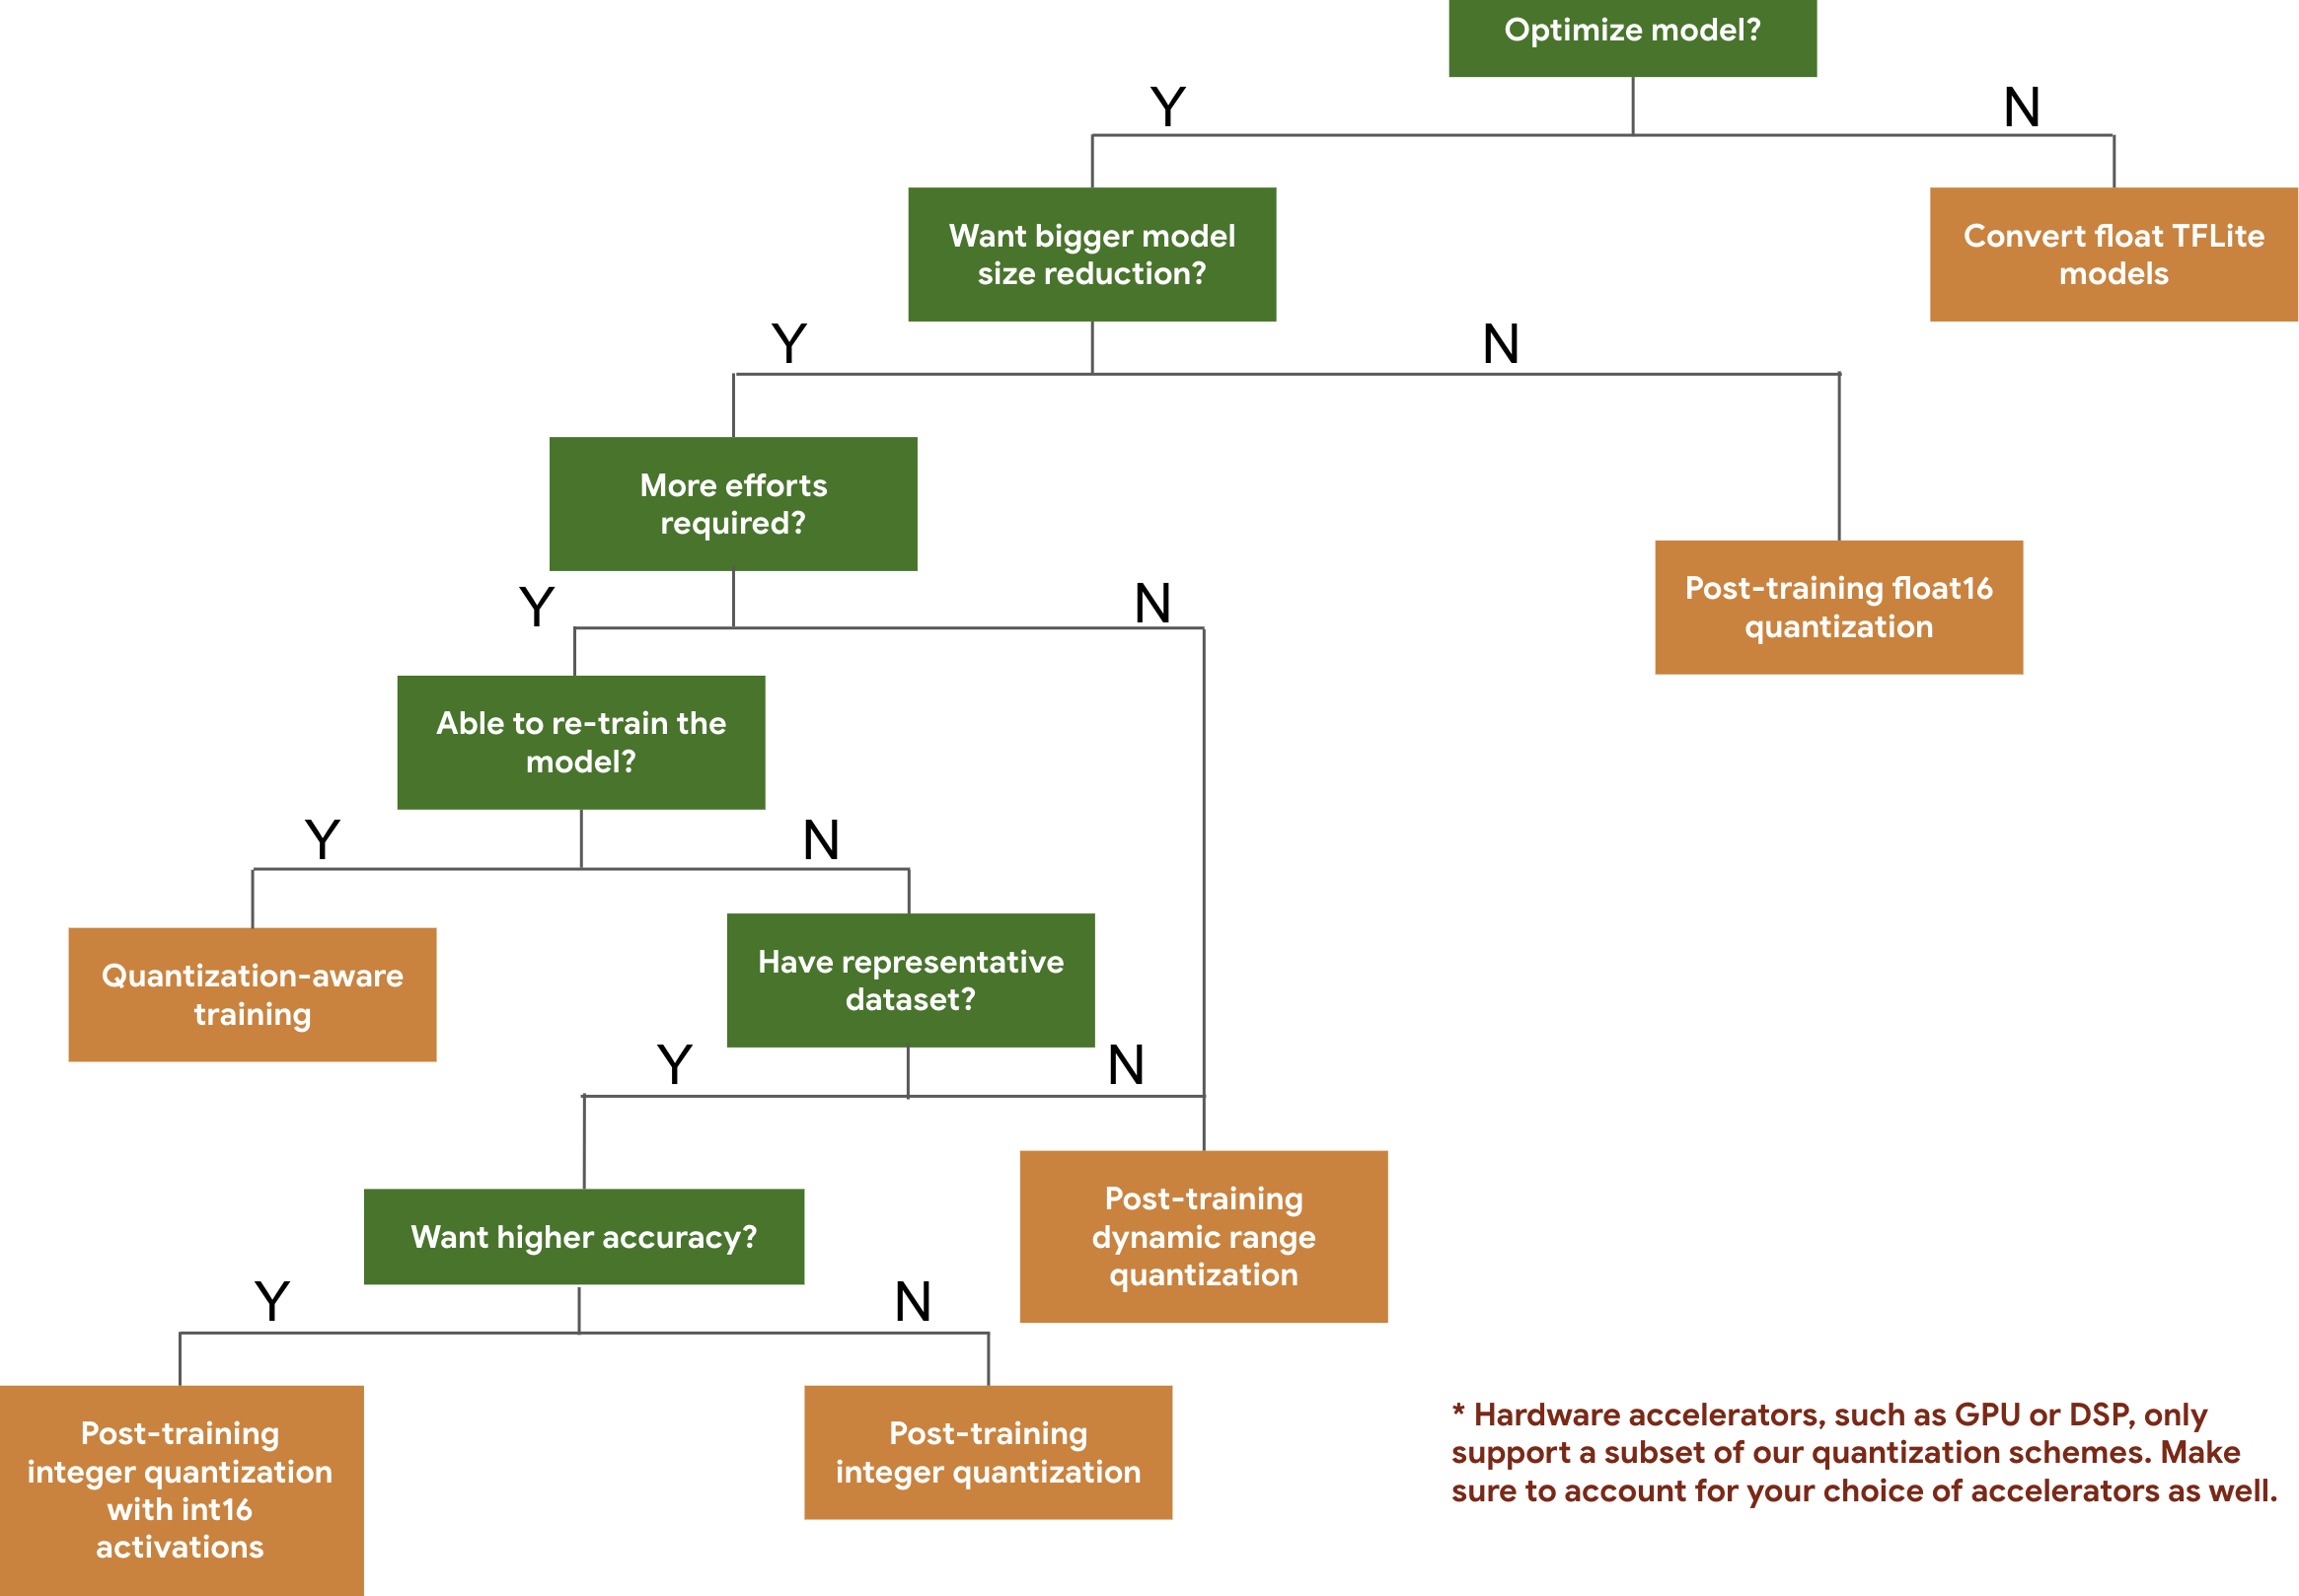
\includegraphics[scale=0.3]{./Figures/tf_quantization_decision_tree.png}
	\caption{Diagrama de árbol de decisiones para el proceso de cuantización\protect\footnotemark.}
	\label{fig:tf_quantization_tree}
\end{figure}
\footnotetext{Imagen tomada de: \url{https://www.tensorflow.org/lite/performance/model_optimization}}

La cuantizacion utilizada para los modelos fue \textit{full integer quantization}, que reduce los picos de memoria utilzados y asegura la compatibilidad con dispositivos de hardware que no pueden utilizar punto flotante. Para este tipo de cuantización se necesito crear un \textit{dataset} representativo, compuesto por un pequeno subconjunto (entre 100 a 500 muestras) del \textit{dataset} de entrenamiento. En ... se expone el codigo utilizado para la conversión de los modelos al formato TensorFlow Lite con cuantización a 8 bits.

La tabla \ref{tab:models_comp} muestra las diferencias entre los tamaños y latencias obtenidas para el modelo O-Net de TensorFlow, TensorFlow Lite sin quantización y TensorFlow Lite con cuantizacion a 8 bits.

\begin{table}[h]
	\centering
	\caption[Modelos comparativa]{Tabla comparativa de O-Net}
	\begin{tabular}{lcc}   
		\toprule
		\textbf{TensorFlow} & \textbf{TensorFlow Lite} & \textbf{TensorFlow Lite int8} \\
		\midrule
		Tamaño (bytes) & 2 V a 15 V & x \\
		Latencia (ms) & 2 V a 15 V & x \\
		\bottomrule
		\hline
	\end{tabular}
	\label{tab:models_comp}
\end{table}

Todo el código para la obtención de los modelos hasta aquí expuesto, las funciones del \textit{pipeline}, las pruebas realizadas a los modelos y el despliegue de estos en el SoC ESP32-S3, se encuentra disponible en el repositorio de acceso público \cite{mtcnn_repo}.

%----------------------------------------------------------------------------------------
\section{Desarrollo del firmware}
El primer paso para el desarrollo del firmware del dispositivo fue la elección de un conjunto de herramientas de software o SDK (\textit{Software Development Kit}, Kit de Desarrollo de software) por sus siglas en inglés. Estas herramientas permitieron implementar código para utilizar de manera eficiente todos los periféricos disponibles en el ESP32-S3. Para este proyecto el SDK utilizado fue ESP-IDF \cite{idf_repo}, las razones de su elección fueron:
\begin{itemize}
	\item Experiencia:
	\item Compatibilidad:
	\item Herramientas:
	\item Soporte:
	\item Documentación:
\end{itemize}

Con el conjunto de herramientas definido, otro aspecto de importancia fue la elección de un entorno de desarrollo para optimizar la escritura y depuración de código. El IDE (\textit{Integrated Development Environment}, Entorno de Desarrollo Integrado) escogido fue Eclipse IDE C/C++, los aspectos más importantes para su elección fueron:
\begin{itemize}
	\item Experiencia:
	\item Herramientas:
	\item Complementos: 
\end{itemize}

Otra herramienta importante para el proceso de desarrollo del firmware fue la utlización de sofware para control de versiones, que permite realizar un seguimiento de los cambios realizados en el código a lo largo del tiempo. Git fue elegido como software de control de versiones, mientras que GitHub como plataforma para alojar el repositorio de Git. Las razones para la elección de ambos son:
\begin{itemize}
	\item Experiencia:
	\item Reutilización de código:
	\item Soporte:
	\item Documentación:
\end{itemize}

Con todas las herramientas de software correctamente seleccionadas, el siguiente paso fue el diseño de la arquitectura del firmware. El firmware desarrollado siguió una arquitectura en capas, donde las capas de niveles más bajos tienen una mayor interacción con el hardware, mientras que las de niveles más altos con la aplicación del usuario. En la figura \ref{fig:fw_layers} se presenta el diagrama en capas del firmware.

\begin{figure}[h]
	\centering
	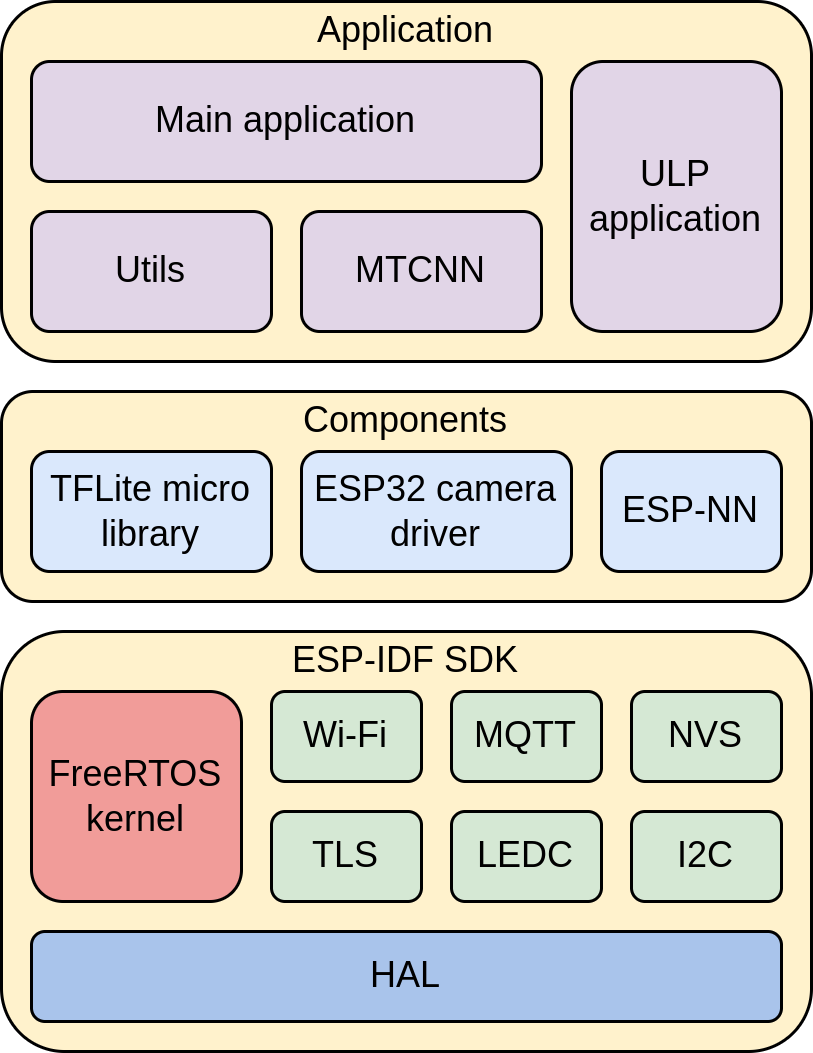
\includegraphics[scale=0.25]{./Figures/fw_layers.png}
	\caption{Diagrama de capas del firmware.}
	\label{fig:fw_layers}
\end{figure}

Las capas expuestas en el diagrama de la figura \ref{fig:fw_layers} son:
\begin{itemize}
	\item ESP-IDF SDK:
	\item \textit{Components}:
	\begin{itemize}
		\item TFLite micro library:
		\item ESP32 camera driver:
		\item ESP-NN:
	\end{itemize}
	\item \textit{Application}:
	\begin{itemize}
		\item \textit{Main application}:
		\item \textit{Main application}:
		\item MTCNN:
		\item \textit{Utils}:
	\end{itemize}
\end{itemize}

El firmware desarrollado cumple con las siguientes tareas: detección facial con TensorFlow Lite para microcontroladores, comunicación con los servicios en la nube y gestión del consumo energético.

\subsection{Deteccion facial con TensorFlow Lite para microontroladores}
En la sección \ref{section3_1} se obtuvieron los modelos para MTCNN en los formatos TensorFlow, TensorFlow Lite y TensorFlow Lite para microcontroladores. El objetivo de esta tarea es obtener imágenes con la cámara del sistema para procesarlas con los modelos de MTCNN y determinar la cantidad  de rostros humanos existentes en cada imagen. El diagrama de flujo de la figura \ref{fig:fw_detect_flow} detalla el proceso de esta tarea.

\begin{figure}[h]
	\centering
	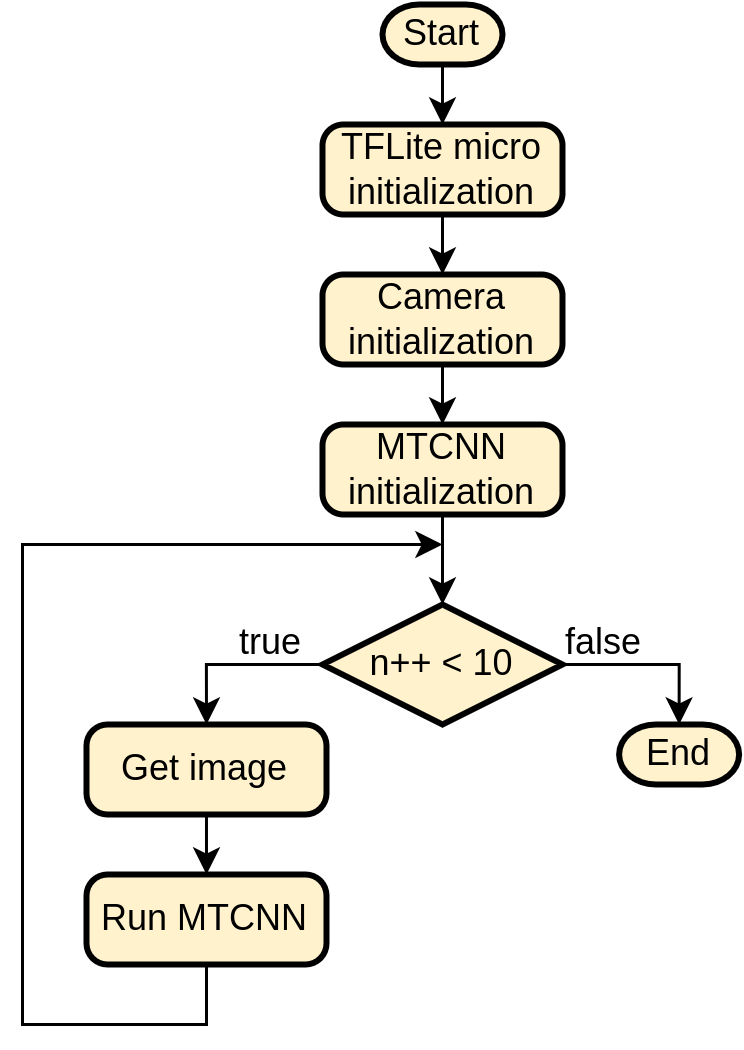
\includegraphics[scale=0.22]{./Figures/fw_detection_flow.png}
	\caption{Diagrama de flujo de la tarea de detección facial.}
	\label{fig:fw_detect_flow}
\end{figure}

El proceso de inicialización de TFLite micro requiere de varios pasos que deben ser seguidos en orden para poder ejecutar los modelos de MTCNN correctamente. En el fragmento de codigo ... se presenta la inicialización para O-Net con TFLite micro.

\begin{lstlisting}[label=cod:tflm_init,caption=Código para inicializar O-Net con TFLite micro.]
/* Map the model into a usable data structure */
const tflite::Model *onet_model = tflite::GetModel(onet_model_data);

/* Reserve memory for the tensors */
uint8_t *tensor_arena = (uint8_t *)heap_caps_malloc(TENSOR_ARENA_SIZE, MALLOC_CAP_SPIRAM | MALLOC_CAP_8BIT);

/* Pull in only the operation implementations needed */
static tflite::MicroMutableOpResolver<10> micro_op_resolver;
micro_op_resolver.AddAveragePool2D();
micro_op_resolver.AddConv2D();
micro_op_resolver.AddPrelu();
micro_op_resolver.AddMaxPool2D();
micro_op_resolver.AddTranspose();
micro_op_resolver.AddFullyConnected();
micro_op_resolver.AddDequantize();
micro_op_resolver.AddDepthwiseConv2D();
micro_op_resolver.AddReshape();
micro_op_resolver.AddSoftmax();

/* Build an interpreter to run the model with */
static tflite::MicroInterpreter static_onet_interpreter(onet_model, micro_op_resolver, tensor_arena, TENSOR_ARENA_SIZE);
onet_interpreter = &static_onet_interpreter;

/* Allocate memory from the tensor_arena for the model's tensors */
onet_interpreter->AllocateTensors();
\end{lstlisting}

Los modelos de P-Net y R-Net se inicializan de la misma forma que O-Net y una cosa a notar es la declaración de los operadores estrictamente necesarios para ejecutar estos modelos en las líneas 9-18. Otra aproximación más sencilla era utilizar \texttt{OpsResolver} para utilizar todos los operadores, pero esto hubiera supuesto una penalización en la cantidad de memoria RAM utilizada. En la figura \ref{fig:fw_tflite_ops} se puede observar una captura de pantalla de una página web generada con la herramienta de visualización de modelos de TensorFlow Lite que se encuentra en el repositorio oficial de TensorFLow Lite para microcontroladores\cite{tflm_repo}, donde se muestran los operadores utilizados por O-Net.

\begin{figure}[h]
	\centering
	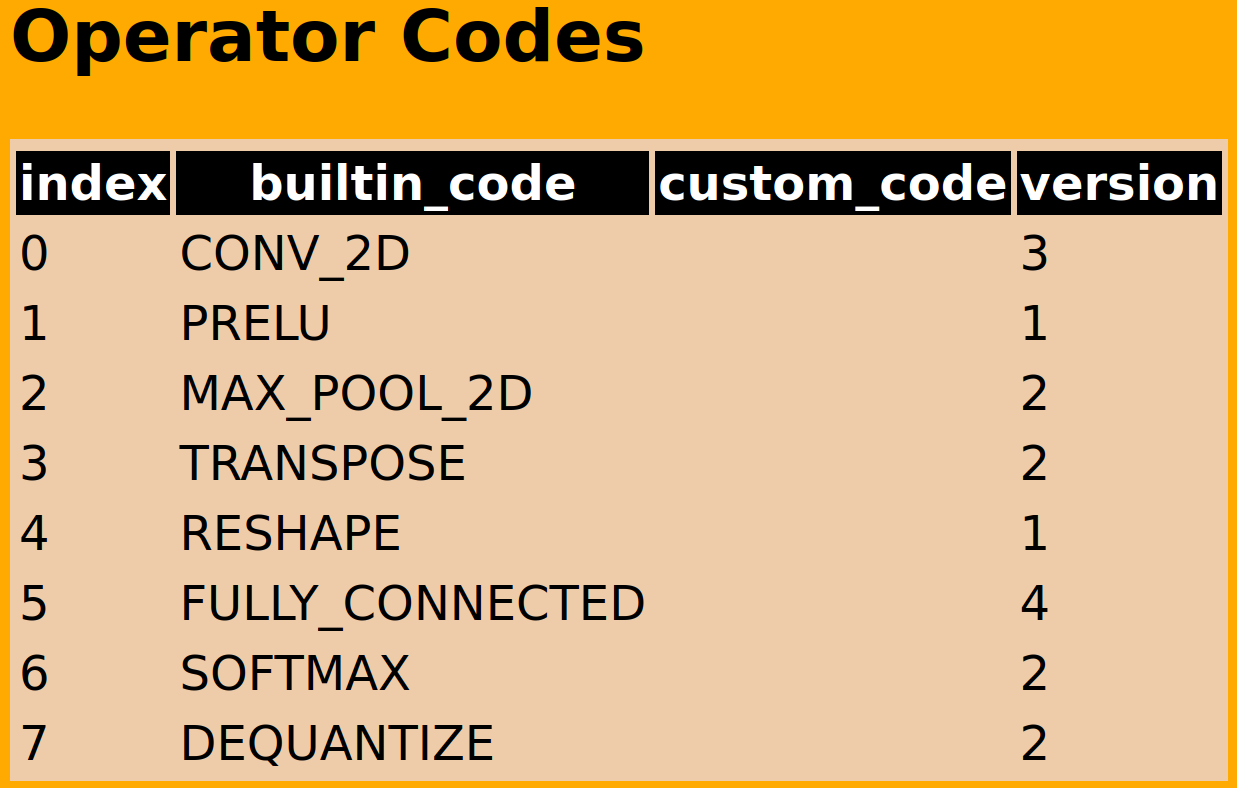
\includegraphics[scale=0.18]{./Figures/fw_tflite_ops.png}
	\caption{Captura de pantalla del detalle del modelo O-Net para TensorFlow Lite.}
	\label{fig:fw_tflite_ops}
\end{figure}

Otro aspecto a destacar es la utilización de la memoria PSRAM (\textit{Pseudo static} RAM, RAM Pseudoestática) para almacenar los tensores utilizados durante la ejecucióin de los modelos de MTCNN. En la línea 5 del fragmento de código ... se puede observar como se reserva memoria en la PSRAM de un tamaño determinado de manera experimental y denominado \texttt{TENSOR\_ARENA\_SIZE}.

Los métodos de MTCNN para inicializarlo y ejecutar sus modelos se encuentran en los archivos \texttt{main/mtcnn.h} y \texttt{mtcnn.cc} del repositorio \cite{mtcnn_repo}. En el fragmento de código ... se pueden observar las estructuras de datos utilizadas por los métodos de MTCNN.

\begin{lstlisting}[label=cod:mtcnn_struct,caption=Estructura de datos de MTCNN.]
typedef struct {
  tflite::MicroInterpreter *interpreter;
  candidate_windows_t candidate_windows;
  bboxes_t bboxes;
} model_data_t;

typedef struct {
  model_data_t pnet[3];
  model_data_t rnet;
  model_data_t onet;
} mtcnn_t;
\end{lstlisting}

Como el tipo de dato \texttt{mtcnn\_t} contiene todos los datos de entrada y salida de los modelos de MTCNN, fue utilizado como parámetro de todas las funciones encargadas de ejecutar los modelos. La función que ejecuta O-Net es \texttt{mtcnn\_run\_onet} y en el fragmento de código ... se puede observar su implementación.

\begin{lstlisting}[label=cod:mtcnn_struct,caption=Función mtcnn\_run\_onet.]
void mtcnn\_run_\onet(mtcnn_t *mtcnn, uint8_t *img, uint16_t img_w, uint16_t img_h) {
  /* Pre-process R-Net ouputs */
  
  /* Feed the model and run it */
  TfLiteTensor *input = mtcnn->interpreter->input(0);
    
  for(int i = 0; i < ONET_SIZE * ONET_SIZE * 3; i++) {
    input->data.int8[i] = ((uint8_t *) onet_image)[i] ^ 0x80;
  }
  
  mtcnn->interpreter->Invoke();
  
  /* Store the scores and offsets output */
  TfLiteTensor *scores = interpreter->output(0);
  
  for(uint8_t j = 0; j < 2; j++) {
    probs_buf[j + (i * 2)] = probs->data.f[j];
  }

  TfLiteTensor *offsets = interpreter->output(1);

  for(uint8_t j = 0; j < 4; j++) {
    offsets_buf[j + (i * 2)] = offsets->data.f[j];
  }
  
  /* Add the candidate windows to the candidate windows array */
  add_candidate_windows();
  
  /* Post-process O-Net ouputs */
}
\end{lstlisting}

\subsection{Comunicación con los servicios en la nube}
Esta tarea fue diseñada para establecer conectividad con los servicios en la nube, más precisamente con el servicio IoT Core de AWS, para transmitir y recibir datos mediante el protocolo MQTT (MQ \textit{Telemetry Transport}, Transporte de Telemetría MQ). El diagrama de flujo de la figura \ref{fig:fw_comm_flow} muestra el proceso que sigue esta tarea.

\begin{figure}[h]
	\centering
	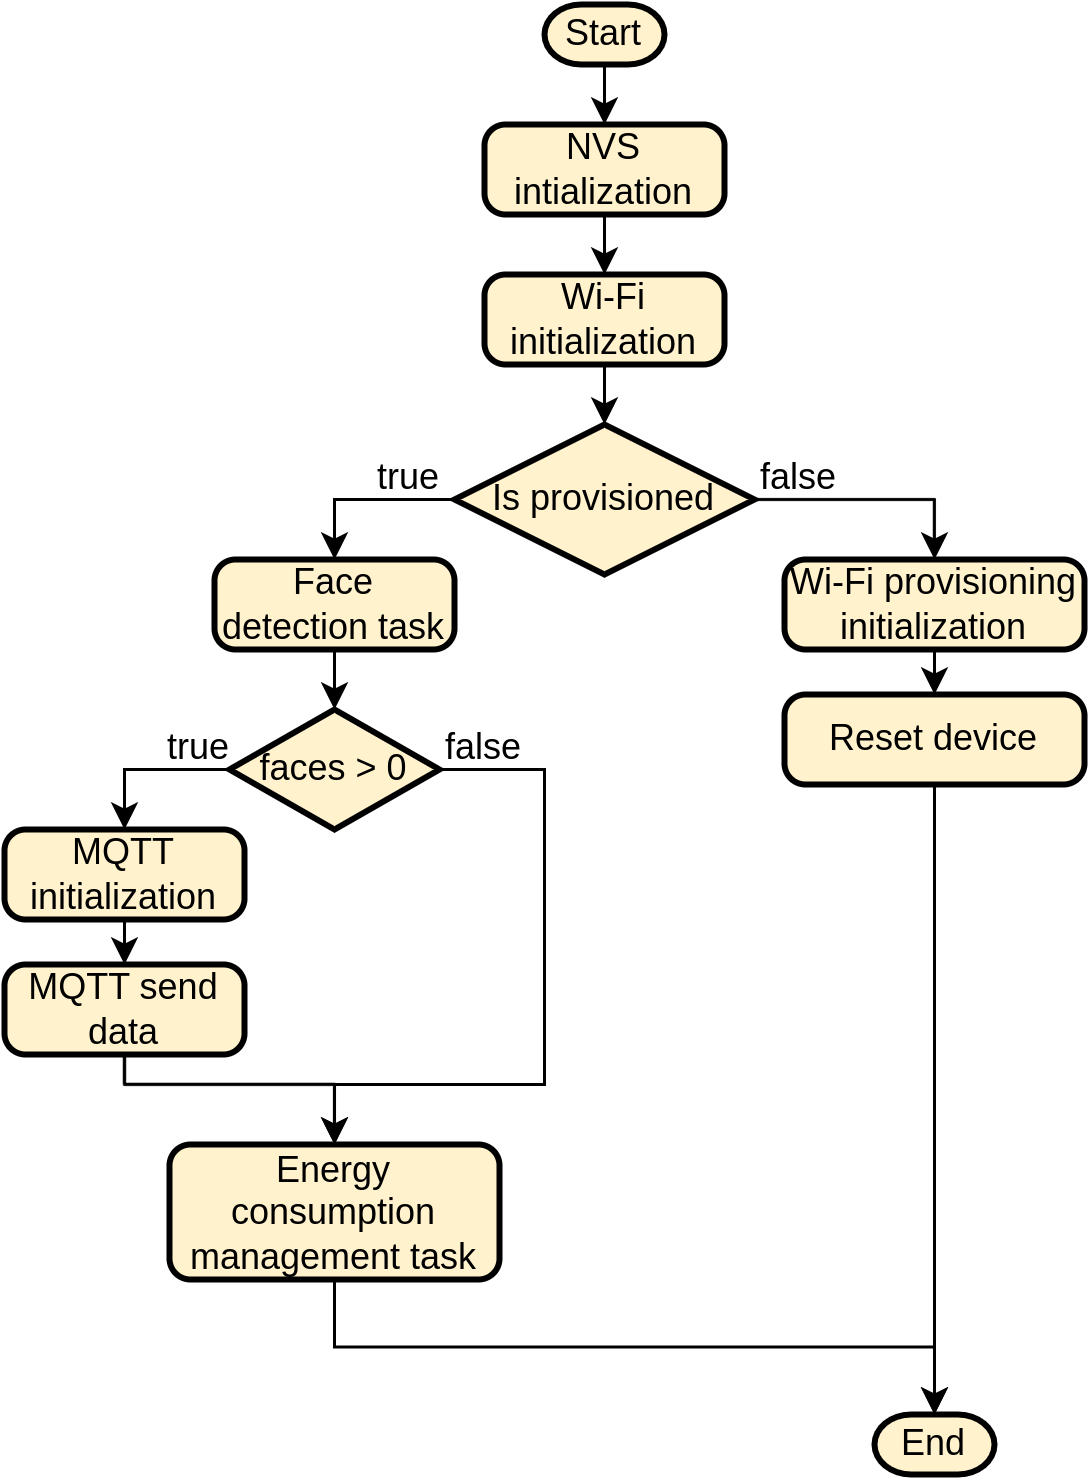
\includegraphics[scale=0.22]{./Figures/fw_comm_flow.png}
	\caption{Diagrama de flujo de la tarea de comunicación con los servicios en la nube.}
	\label{fig:fw_comm_flow}
\end{figure}

El digrama de la figura \ref{fig:fw_comm_flow} empieza con la inicialización de la memoria NVS y el perférico Wi-Fi en modo punto de acceso y estación, para después establecer si el dispositivo debe ejecutar el proceso de provisionamiento de credenciales Wi-Fi o en cambio ejecutar la tarea de detección facial y transmitir los datos generados. El provisionamiento de credenciales Wi-Fi utiliza un protocolo de comunicación llamado protocomm (\textit{protocol communication}) de Espressif \cite{protocomm_doc} y corre sobre Wi-Fi en modo SoftAP (\textit{Software enabled Access Point}, Punto de Acceso habilitado por Software). En el fragmento de código ... se exhiben las línea de código para la inicializacion del provisionamiento Wi-Fi.

\begin{lstlisting}[label=cod:mtcnn_struct,caption=Función mtcnn\_run\_onet.]
/* Initalize Wi-Fi provisioning over SoftAP */
wifi_prov_mgr_config_t prov_config = {
  .scheme = wifi_prov_scheme_softap,
  .scheme_event_handler = WIFI_PROV_EVENT_HANDLER_NONE,
  .app_event_handler = WIFI_PROV_EVENT_HANDLER_NONE
};

ESP_ERROR_CHECK(wifi_prov_mgr_init(prov_config));
\end{lstlisting}

Cuando se ejecuta la tarea de detección facial pueden o no detectarse rostros humanos en la imágenes obtenidas por la cámara, cuando uno más rostros son detectados esta información se transmite por MQTT. AWS IoT Core dispone de un \textit{broker} MQTT que implementa TLS (\textit{Transport Layer Security}, Seguridad de la Capa de Transporte) \cite{tls_doc} para brindar seguridad en el intercambio de mensajes, por tanto, la autenticacíon y cifrado de datos necesita de certificados y llaves para llevarse a cabo. La llave privada y el certificado del dispositivo son generados en la plataforma AWS IoT Core y deben quedar grabadas en la memoria del ESP32-S3 para que puedan ser utilizadas en el código. La forma más simple de utilizar la llave y el certificado es añadirlas al binario de la aplicación durante el proceso de compilación, en la figura \ref{fig:fw_parttab1} se observa un diagrama representativo de la distribución de la memoria del ESP32-S3, donde los valores encima de los bloques son las posiciones de memoria donde se encuentran las particiones y los valores que se encuentran por debajo son la cantidad de memoria utilizada.

\begin{figure}[h]
	\centering
	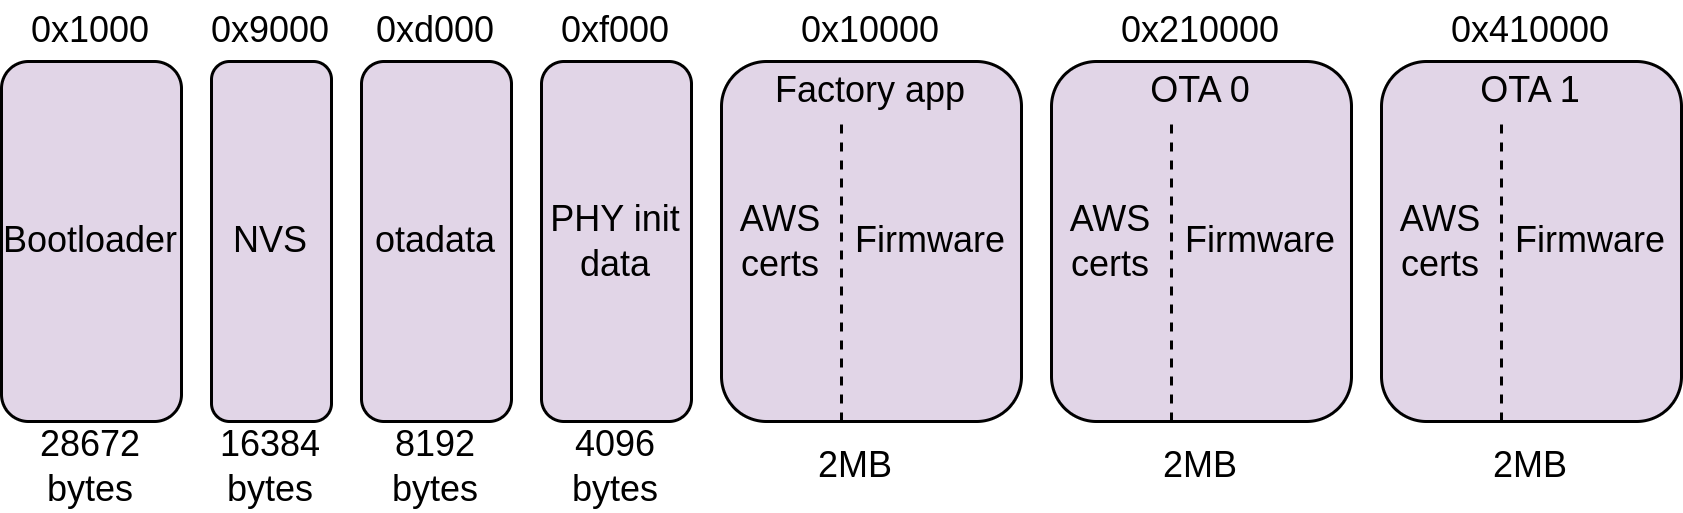
\includegraphics[scale=0.22]{./Figures/fw_parttab1.png}
	\caption{Diagrama representativo de la memoria del ESP32-S3.}
	\label{fig:fw_parttab1}
\end{figure}

En el diagrama de la figura \ref{fig:fw_parttab1} se puede observar un problema no menor con respecto a al proceso de actualizaciones OTA, que las actualizaciones sobreescribirán tanto el \textit{firmware} como el certificado y llave privada del dipositivo. Esto no sería problemático para un solo dispotivo, pero si existieran más dispositivos establecerian conexión con AWS IoT Core con el mismo certificado y llave privada, lo que supondría una grave falla de seguridad de la información. Para corregir esta falla de seguridad se optó por generar llaves y certificados únicos para cada dispositivo, y grabarlos en la memoria NVS en un \textit{namespace} llamado "certs", de esta forma el proceso de actualización OTA solo sobreescribirá el \textit{firmware} más no el certificado ni la llave. En la figura \ref{fig:fw_parttab2} se muestra el diagrama representativo de la memoria del ESP32-S3 utilziado en este trabajo.

\begin{figure}[h]
	\centering
	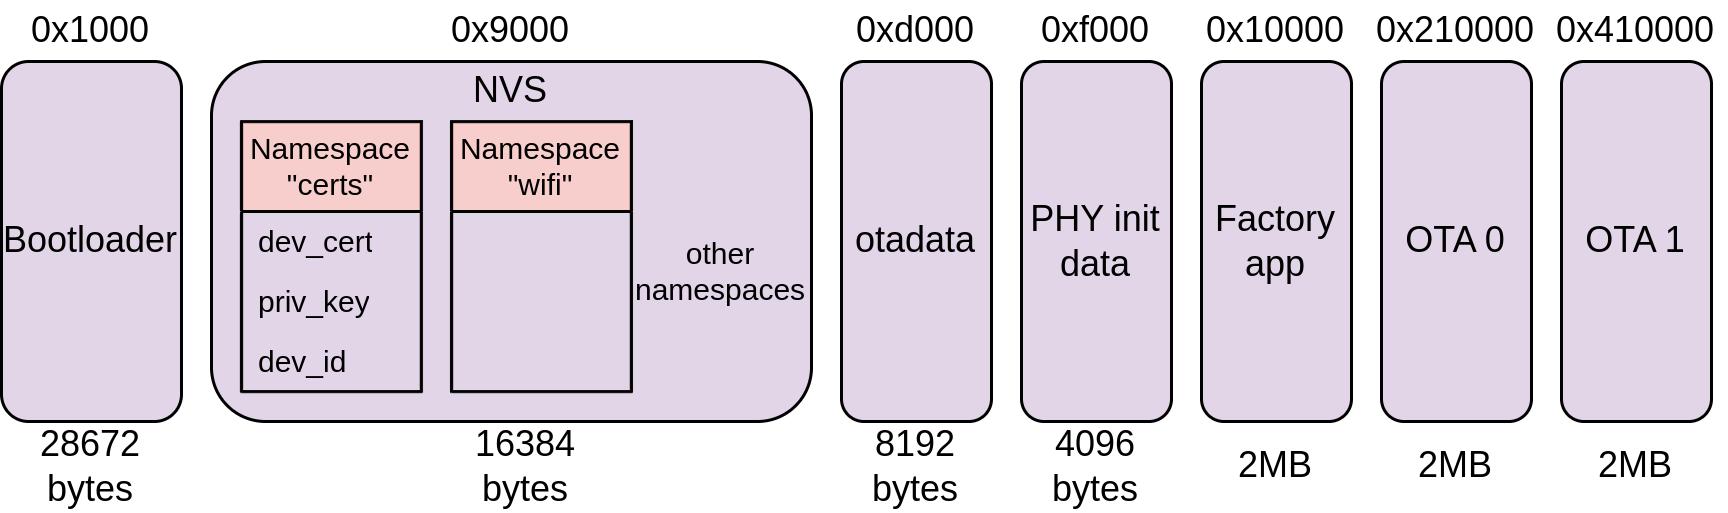
\includegraphics[scale=0.22]{./Figures/fw_parttab2.png}
	\caption{Diagrama representativo de la memoria del ESP32-S3.}
	\label{fig:fw_parttab2}
\end{figure}

La inicialización de MQTT en el código utiliza una estructura de datos donde algunoss campos debens ser asignados al certificado del dispositivo y la llave privada en formato de cadena de caracteres. En los fragmentos de codigo ... se exhibe la función para obtener una cadena de caracteres de la NVS y la inicialización de MQTT en modo cliente.

\begin{lstlisting}[label=cod:mtcnn_struct,caption=Función para cargar una cadena de caracteres de la NVS.]
esp_err_t load_string_from_nvs(const char * namespace_name, const char *key, char **value) {
  esp_err_t ret = ESP_OK;
  nvs_handle_t nvs_handle;
  size_t value_size;

  /* Open the name space to read and write */
  ret = nvs_open(namespace_name, NVS_READONLY, &nvs_handle);

  if (ret != ESP_OK) {
	ESP_LOGE(TAG, "Error opening namespace %s", namespace_name);
	return ret;
  }

  /* Get value size */
  ret = nvs_get_str(nvs_handle, key, NULL, &value_size);

  if (ret != ESP_OK){
	ESP_LOGE(TAG, "Failed to get size of key: %s", key);
    return ret;
  }

  /* Allocate memory and get value */
  *value = (char *)malloc(value_size);
  ret = nvs_get_str(nvs_handle, key, * value, &value_size);

  if (ret != ESP_OK){
	 ESP_LOGE(TAG, "Failed to load key: %s", key);
     return ret;
  }

  /* Close NVS and return */
  nvs_close(nvs_handle);
  return ret;
}
\end{lstlisting}

\begin{lstlisting}[label=cod:mtcnn_struct,caption=Código para inicializar MQTT en modo cliente.]
/* CA certificate is embedded in the binary application */
extern const char amazon_root_ca1_pem_start[] asm("_binary_amazon_root_ca1_pem_start");

/* Get device certificate and private key from NVS */
char *device_cert = NULL;
char *priv_key = NULL;

load_string_from_nvs("certs", "dev_cert", &dev_cert);
load_string_from_nvs("certs", "priv_key", &priv_key);

/* Fill MQTT client configuration */
const esp_mqtt_client_config_t mqtt_config = {
  .broker = {
    .address = {
      .uri = BROKER_URL, /* Broker address in port 8883 */
    },
	.verification = {
      .certificate = (const char *)amazon_root_ca1_pem_start,
    },
  },
  .credentials = {
    .authentication = {
      .certificate = (const char *)dev_cert,
      .key = (const char *)priv_key
    },
  },
};

/* Initialize MQTT client */
mqtt_client = esp_mqtt_client_init(&mqtt_config);
\end{lstlisting}

\subsection{Gestión del consumo energético}
TBD
%----------------------------------------------------------------------------------------
\section{Procesamiento y visualización en la nube}
Otro aspecto de importancia en este trabajo fue la integración del sistema embebido con los servicios en la nube responsables de procesar los datos entrantes y mostrarlos en un \textit{dashboard} adecuado para que los usuarios finales puedan visualizar la actividad de los dispositivos. En la figura \ref{fig:cc_diagram} se puede observar la arquitectura de los servicios en la nube.

\begin{figure}[h]
	\centering
	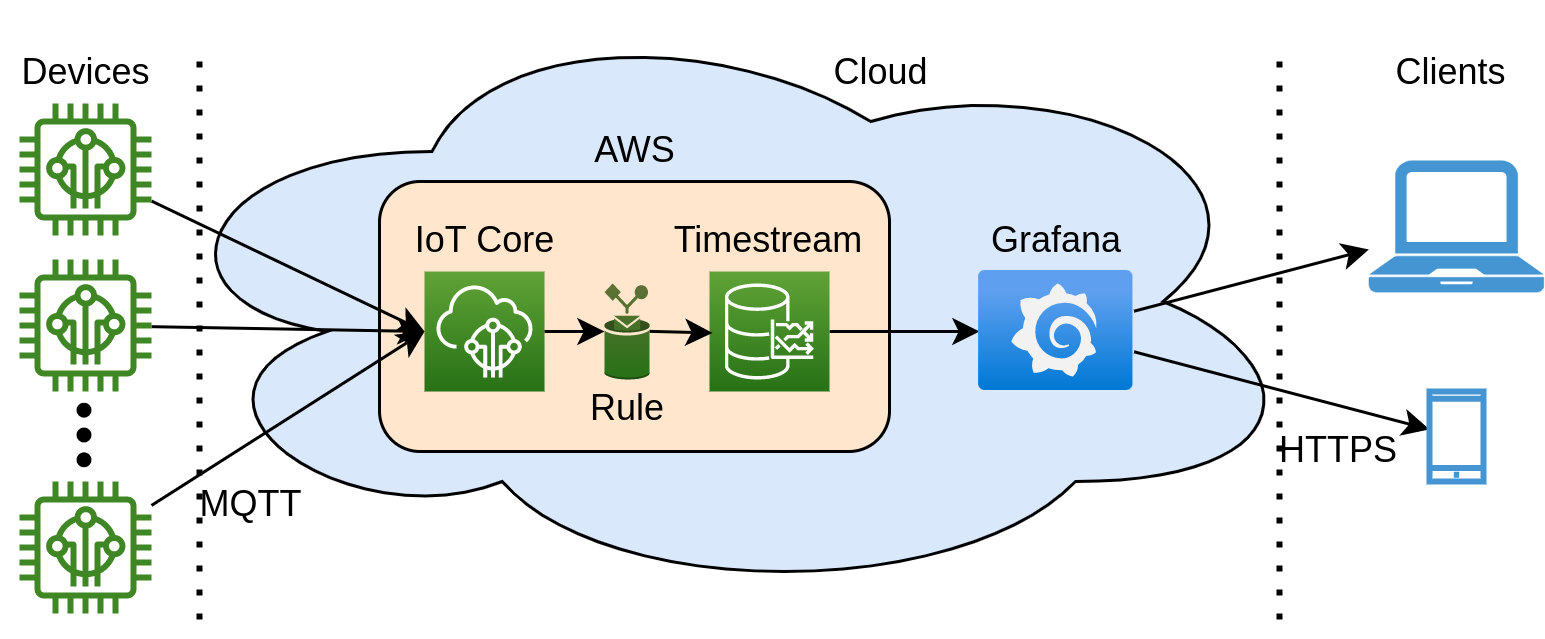
\includegraphics[scale=0.22]{./Figures/cc_diagram.png}
	\caption{Arquitectura de los servicios en la nube.}
	\label{fig:cc_diagram}
\end{figure}

De la figura \ref{fig:cc_diagram} se infiere que los datos generados por los dispositivos son transmitidos por MQTT hacia IoT Core, donde meidiante un \textit{rule} se extrae la información relevante y se guarda en una base de datos de TimeStream. Los datos de TimeStream son utilizados para crear un \textit{dashboard} en Grafana, que puede ser accedido por diferentes tipos de dipositivos con un navegador web mediante el protocolo HTTPS.

\subsection{Gestión de dispositivos con IoT Core}
\label{subsection3_3_1}


\subsection{Bases de datos de series temporales con TimeStream}


\subsection{Visualiación de datos con Grafana}




